\chapter{Theoretical Background}
\label{cap-background}

As described in \textcite{fowler2018refactoring}, refactoring is a design improvement after writing a code. Refactoring opportunities may arise throughout the project's development regardless of how the project was carried out, especially in systems developed by teams.

Refactoring seeks to remove code smells encountered in software development; when software becomes mature and evolves, two conflicts arise: i) the software needs to fulfill all requirements, and ii) The software's reusability. Implementing new functionality in software without refactoring is possible, but it will eventually take great effort \cite{Gamma2009}.

Refactoring can facilitate the implementation of new requirements, modularize overloaded classes, and find methods and unnecessary classes. Different types of refactoring exist, such as techniques or methods based on design patterns. \textcite{fowler2018refactoring} is one of the most known authors. He created a catalog separating the refactorings into seven (7) groups and making it available for consultation. Fowler's online catalog encompasses the refactorings described in his two books: Refactoring: Improving the Design of Existing Code \cite{fowler2018refactoring} and Refactoring: Ruby Edition \cite{fields2009refactoring}. 

Refactoring by designing pattern-based methods examines the source code for insertion points to apply patterns. This refactoring aims mainly at maintainability, readability, and reusability. Several authors propose their pattern-based refactoring methods, such as \textcite{cinneide2000automated}, \textcite{Gamma2009}, and \textcite{ouni2017more}.

This chapter has information about the research background. \Cref{sec-importance} discuss the importance of refactoring. \Cref{sec-methods} describes the application of refactoring. \Cref{sec-tools} exemplifies the refactoring methods and the explanations of its functionalities and tools. \Cref{sub-rmt} talks about the RMT functionality. \Cref{sub-architecture} describes the architecture of the tool. \Cref{subsub-internal} talks about the internal functionality of RMT. \Cref{sub-usage} shows how to use the tool. \Cref{subsub-limitation} discusses the limitations encountered using the tool. \Cref{sec-microservices} explain about microservices. \Cref{sec2-remarks} includes the final considerations.

\section{Importance of Software Refactoring}
\label{sec-importance}
\textcite{fowler2018refactoring} describes that the first step in refactoring is to create automated tests, such as unit tests. The tests help to avoid creating bugs by guaranteeing that the behavior does not change, as any code change could also change the code behavior; humans may make mistakes and cause severe problems in production. In system production, maintainability is a significant factor that influences costs, and one of the proposed solutions to reduce it is to increase software quality. 

Refactoring can be applied to the development process to increase software quality, forcing the programmer to find bad smells (a characteristic of the code that indicates an issue) \cite{Wilking2007}. 
In the study of \textcite{szHoke2017empirical}, six systems were analyzed to verify the effectiveness of software refactoring aimed at maintainability. To obtain data before refactoring, \textcite{szHoke2017empirical} analyzed all systems using a code analyzer called the SourcerMeter tool based on the Columbus tool \cite{ferenc2002}. Refactorings were performed manually, and developers were informed of all the data and the list of problematic code fragments. 

In this study, developers analyzed 2.5 million lines and performed 732 code revisions, of which 315 were refactorings and 1,273 refactoring operations. After finishing the analysis, \textcite{szHoke2017empirical} found that refactoring improved maintainability and that the tool improved 5 of the six systems tested. In conclusion, the study shows that refactoring improves maintainability, which helps to meet future software requirements.

\subsection{Methods to Apply refactoring}
\label{sub-methods}
As mentioned, we can apply refactoring techniques and methods based on design patterns. Refactoring by techniques is common and can be found in leading IDEs, such as Eclipse and IntelliJ, which provide automatic refactorings based on the model created by \textcite{fowler2018refactoring}. 

Several authors propose software refactoring methods applying patterns, each performed differently in refactorings using pattern-based design methods. Some of these authors are \textcite{liu2014automated}, \textcite{zafeiris2017automated}, \textcite{cinneide2000automated}, and \cite{ouni2017more}. 
These refactoring methods seek to find the point of insertion of the pattern in the source code. The technique searches for source code to find where to implement design patterns to improve code maintainability, readability, and reusability. 

Unlike technical refactoring, design pattern-based refactoring looks for parts of the code where a design pattern can be applied. Using a design pattern is very important because it makes the evolution of the software more natural and does not create problems when implementing new requirements. Several project patterns have different functionality, such as the factory method, proxy, observer, adapter, visitor, builder, and others \cite{Gamma2009}). 

As described in the mapping performed by \textcite{beluzzo2018abordagem}, several authors propose methods for refactorings based on design patterns. For example, in the Moore method and Minipatterns and Minitransformations, there is a tool for each implementation process. If the developer wants to refactor his source code, he has to run n tools, where n is the total number of methods.

The focus of refactoring by design patterns differs from refactoring by techniques. Refactoring by design patterns tries to find a way to make a system easy to "update." Software that is difficult to update can cost the company a lot in value and need for new clients and competitiveness with other companies \cite{cinneide2000automated}.

\subsection{Methods and Tools for Refactoring Based on Design Patterns}
\label{sec-tools}

As mentioned, \textcite{beluzzo2018abordagem} identified methods for detecting and involving design patterns as described in \Cref{tab-articles}.


\begin{tabframed}[!htbp]
\caption{Articles with design patterns methods}
\label{tab-articles}
\begin{tabularx}{\textwidth}{|e{}@{},{}@{}|p{3cm}|p{8cm}|c|c@{}|}
%% Cabeçalho da primeira página
\toprule%
\multicolumn{1}{|@{}c|}{\textbf{Key}}             &
\multicolumn{1}{c|}{\textbf{Author}}             &
\multicolumn{1}{c|}{\textbf{Title}}              &
\multicolumn{1}{c|}{\textbf{Year}}               &
\multicolumn{1}{c@{}|}{\textbf{Has Tool}}        \\
\midrule%
A1  & \citeauthor*{GAITANI201533}            & Automated refactoring to the Null Object design pattern                                                             & 2015 & Yes      \\
A2  & \citeauthor*{CHRISTOPOULOU20121201}    & Automated refactoring to the Strategy design pattern                                                                & 2012 & Yes      \\
A3  & \citeauthor*{zafeiris2017automated}           & Automated refactoring of super-class method invocations to the Template Method design pattern                       & 2017 & Yes      \\
A4  & \citeauthor*{CINNEIDE2015}             & A multi-objective refactoring approach to introduce design patterns and fix anti-patterns                           & 2015 & Yes      \\
A5  & \citeauthor*{cinneide2001automated}    & Automated application of design patterns: a refactoring approach                                                    & 2001 & Yes      \\
A6  & \citeauthor*{cinneide792644}           & A Methodology for the automated introduction of design patterns                                                     & 1999 & Yes      \\
A7  & \citeauthor*{mens972774}               & A declarative evolution framework for object-oriented design patterns                                               & 2001 & Yes      \\
A8  & \citeauthor*{sang1183003}              & An automated refactoring approach to design pattern-based program transformations in Java programs                  & 2002 & Yes      \\
A9  & \citeauthor*{Cinneide602499}           & Automated Software Evolution Towards Design Patterns                                                                & 2001 & Yes      \\
A10 & \citeauthor*{cinneide337612}           & Automated refactoring to introduce design patterns                                                                  & 2000 & Yes      \\
A11 & \citeauthor*{Liu2014}                  & Automated pattern-directed refactoring for complex conditional statements                                           & 2014 & No       \\
A12 & \citeauthor*{ram2004detecting}         & Detecting Intent Aspects from Code to Apply Design Patterns in Refactoring: An Approach Towards a Refactoring Tool  & 2004 & Yes      \\
A13 & \citeauthor*{hotta6178876}             & Identifying, tailoring and suggesting form template method refactoring Opportunities with program dependence graph. & 2012 & Yes      \\
A14 & \citeauthor*{rajesh1013988}            & JIAD: A tool to infer design patterns in refactoring                                                                & 2004 & Yes      \\
A15 & \citeauthor*{ouni2017more}             & MORE: A multi-objective refactoring recommendation approach to introducing design patterns and fixing code smells   & 2017 & Yes      \\
A16 & \citeauthor*{eden632834}               & Precise specification and automatic application of design patterns                                                  & 1997 & No       \\
A17 & \citeauthor*{kerievsky2005refactoring} & Refactoring to Patterns                                                                                             & 2008 & No       \\
A18 & \citeauthor*{kim7332467}               & Scripting parametric refactorings in java to retrofit design patterns                                               & 2015 & No       \\
A19 & \citeauthor*{kim2014scripting}         & Scripting Refactorings in Java to Introduce Design Patterns                                                         & 2014 & Yes      \\
A20 & \citeauthor*{juillerat4362900}         & Toward an implementation of the ”Form Template Method” Refactoring                                                  & 2007 & Yes      \\
A21 & \citeauthor*{ajouli6619484}            & Transformations between composite and visitor implementations in Java                                               & 2013 & Yes     \\
\bottomrule%
\end{tabularx}
\SourceOrNote{adapted from \textcite{beluzzo2018abordagem}}
\end{tabframed}
\FloatBarrier

Each article has methods to recognize design pattern insertions, but not every article has a tool to apply it, as described in \Cref{tab-articles}. \textcite{beluzzo2018abordagem} searched for the articles until 2018, when his work was published; a new search was carried out with the same search strings and libraries from 2019 to 2023, and no new work was found.

Some steps should be taken to refactor the code and apply transformations, as refactoring is not a straightforward technique and may vary by who is using it. That is why the authors have taken different approaches to refactoring listed in \Cref{tab-refactoring}.

\begin{table}[!htbp]
\caption{Refactoring Types}%
\label{tab-refactoring}
\begin{tabularx}{\textwidth}{e{},{}@{}lX@{}}
\toprule%
\multicolumn{1}{@{}c}{\textbf{Keys}}  &
\multicolumn{1}{c@{}}{\textbf{Types}} \\
\midrule%
A15, A10, A9, A6, A5 & MiniTransformations                                        \\
A2, A11              & Conditional Expression Refactorings                        \\
A12, A14             & Intent Aspects Refactoring*                                \\
A18, A19             & Reflective Refactorings                                    \\
A4, A15, A21         & Composite to Visitor and Visitor to Composite Refactorings \\
A4, A7, A15          & Role based Refactorings                                    \\
\bottomrule%
\end{tabularx}
\SourceOrNote{adapted from \textcite{beluzzo2018abordagem}}
\end{table}
\FloatBarrier


A refactoring type will apply to the code for every work, as described in \Cref{tab-refactoring}.

I) Minitransformations are minitransformations that are simple modifications to the code. By grouping these transformations in the right way, a design pattern is created \cite{cinneide2001automated}. II) Reflective Refactoring is based on code reflections, a technique that allows the code to be changed on runtime. It is good to emphasize that there are no pre-refactoring implementations with reflections; they are a method to implement the refactorings \cite{beluzzo2018abordagem}. III) Role Role-based refactoring is defined by a group of roles corresponding to the pattern participants and applying those roles to the refactor, obtaining the design pattern \cite{mens972774}. IV) Intent aspects are aspects of software susceptible to pattern refactoring, formed by a group of rules for each pattern\cite{ram2004detecting}. V) Composite to Visitor and Visitor to Composite: focus only on the transition between each pattern \cite{beluzzo2018abordagem}. VI) Conditional Expression Refactorings: focus on the code's conditional expressions and conditional branches to refactor. \cite{CHRISTOPOULOU20121201}

As shown in \Cref{tab-articles}, most articles have tools developed to apply the methods described above, working in an automatic or semi-automatic manner.

\begin{table}[!htbp]
\caption{Developed tools}%
\label{tab-tools}
\begin{tabularx}{\textwidth}{e{},{}@{}lX@{}}
\toprule%
\multicolumn{1}{@{}c}{\textbf{Keys}}  &
\multicolumn{1}{c@{}}{\textbf{Tools}} \\
\midrule%
A2, A3         & JDeodorant                   \\
A4             & MORE                         \\
A6, A7, A8, A9 & Prototype\textbf{*}          \\
A5, A10        & Design Pattern Tool          \\
A13            & Creios                       \\
A12, A15       & JIAD                         \\
A15            & MORE                         \\
A11, A19, A20  & Eclipse Plugin\textbf{*}     \\
A21            & JHotDraw                     \\
\bottomrule%
\end{tabularx}
\SourceOrNote{adapted from \textcite{beluzzo2018abordagem}}
\end{table}
\FloatBarrier

In \Cref{tab-tools}, the developed tools are listed by name; the row marked with an asterisk means that the tool is a prototype or an eclipse plugin; the other articles were created or updated of specific tools\cite{beluzzo2018abordagem}.

The tool creation is necessary because manual refactoring, the process some developers use, can introduce errors to the code and even change the system's functionality. This problem occurs because developers are not prepared to perform a refactoring \cite{ge2012reconciling}.

Manual refactoring requires reviewing the entire code and can take time. For this reason, tools facilitate the application of refactorings, which can identify bad smells or identify and refactor the source code, as created by \textcite{beluzzo2018abordagem}.

\textcite{beluzzo2018abordagem} performed a mapping to find refactoring techniques and several tools have already been developed to perform refactorings. Such as Elbereth \cite{korman1998elbereth}, which automates some code extraction refactorings, encompassing method extraction (Extract Method), abstract superclasses, replacement of an existing class, and addition of a new subclass.

To improve the interaction with the user for the application of refactoring, \cite{murphy2008breaking} created a tool that is fast, resistant to errors, and pleasant to use. To make the tool enjoyable, they implemented markings in the code produced by rectangles, arrows, and coloring parts of the code. These three markings show the user cleanly where and what the problem is so that refactorings can be applied.
Some tools contain a graphical interface and iteration with the user, such as \textcite{rani2014detection}, where the intent is to detect bad smells. This tool was developed in C\# and finds terrible smells such as the long method, large class, lazy class, and comment lines. Discovering smells in code written in JAVA and .net. 

Many code refactoring tools are based on the catalog of refactorings created by \cite{fowler2018refactoring}. However, other authors propose new refactorings. However, most authors agree that manually performed refactoring is time-consuming and challenging without creating new smells in the code. They were making tools for this reason.

\cite{murphy2008breaking}, together with eight software developers with different work experiences, used the GostFactor tool to assist in refactoring. They observed that this process decreased errors in the refactoring application by 23.3\%.

The RMT tool created by \textcite{beluzzo2018abordagem} allows one to integrate design pattern insertion and detection methods in a single environment. The tool has an iteration with the user to let them know what will happen in the code after refactoring and, simultaneously, if the refactoring will improve the code. The work of \textcite{sangeetha2019empirical} does not describe how the implemented tool works but uses it to test and validate the techniques used. The RMT was created to implement the methods cited above. \textcite{beluzzo2018abordagem} implemented two methods, allowing the tool to extend to as many methods as possible.

\subsection{RMT}
\label{sub-rmt}

The RMT (Refactoring and Measurement Tool) tool was created to detect design pattern insertion points using the methods selected by the author \cite{beluzzo2018abordagem}. \textcite{zafeiris2017automated} and \textcite{liu2014automated} developed the refactoring methods already implemented. The method of \textcite{zafeiris2017automated} covers refactoring for the Template Method pattern, and the method by \textcite{liu2014automated} covers two patterns: Strategy and Factory Method.

\begin{figure}[ht!]
\SetCaptionWidth{\textwidth}
\caption{RMT use case}
\label{fig-usecase}
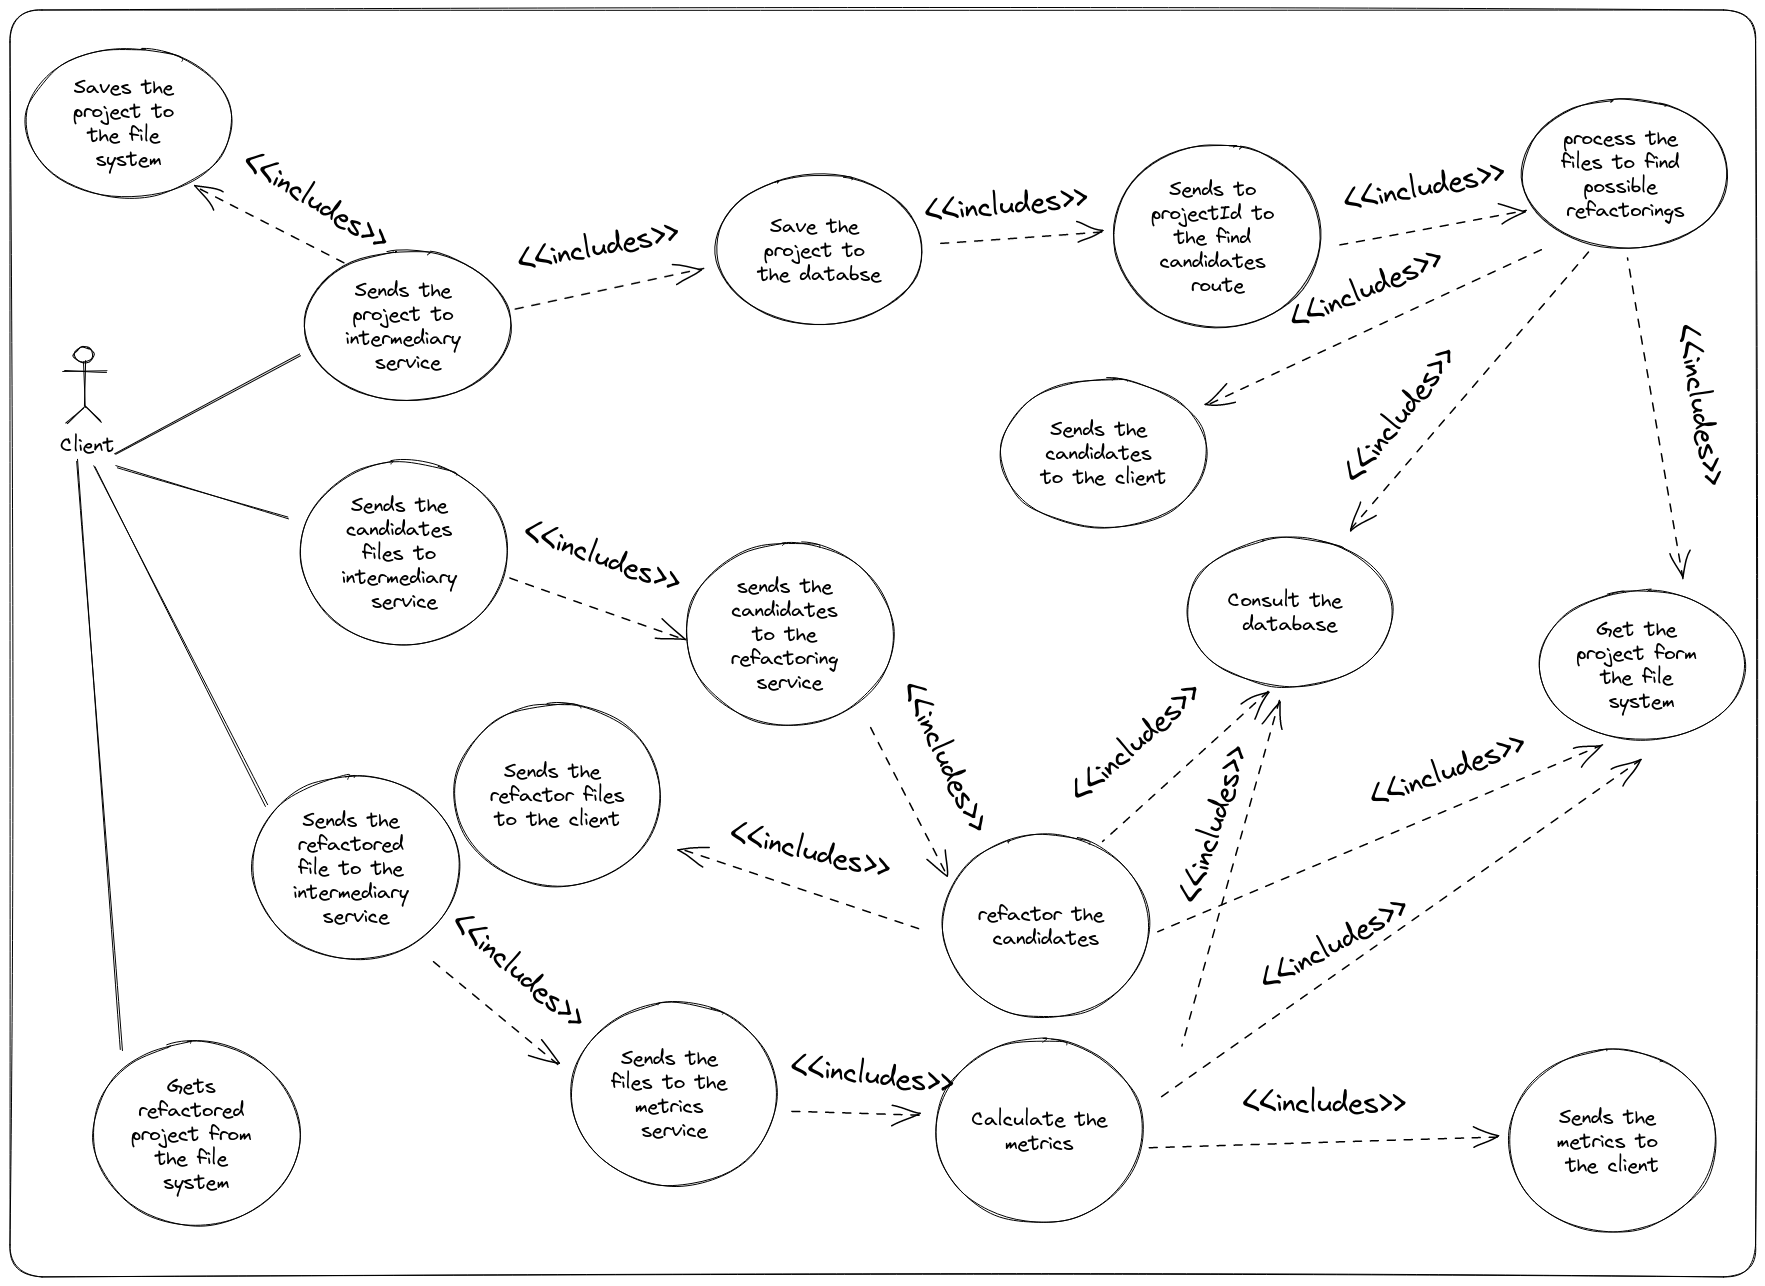
\includegraphics[width =\textwidth]{Chapter-2/Figures/usecase.png}
\SourceOrNote{Own authorship (2023)}
\end{figure}
\FloatBarrier

The use case diagram describes the tool's functionality for the user in \Cref{fig-usecase}; the client starts by uploading the project and searching for candidates; if any applicable method is found, the metric is calculated. On the interface, the client can select which class he wants to refactor, if any, and then refactor.

\subsubsection{RMT Architecture}
\label{sub-architecture}

 In addition to applying the refactorings, the tool uses the CK metrics extractor \cite{ck}, which encompasses the metrics of the depth of the inheritance tree (PAH), the cyclomatic complexity (CC), and the size of the program in lines of code (TPLC). After selecting a project to be refactored, the metrics are applied to demonstrate the effects of refactorings on the user source code. The external quality attributes used were maintainability, reliability, and reusability.

The user iteration within the Client App can be performed independently since it communicates with the Intermediary Service, which provides the service that communicates the user layer (Client) with the processing layer (Services). The Intermediary Service uses a REST request for each service, one for the Metrics Service and one for the Detection Methods Service.

The model created by \textcite{beluzzo2018abordagem} also proposes a region's system structure with higher fault tolerance because the more regions there are, the more members for processing will exist. Another factor \textcite{beluzzo2018abordagem} describes high availability, in which regions should be placed on different servers, preventing overload and natural disasters. \Cref{fig-architecture} represents the regional divisions and application services.

\begin{figure}[ht!]
\SetCaptionWidth{\textwidth}
\caption{RMT architecture diagram}
\label{fig-architecture}
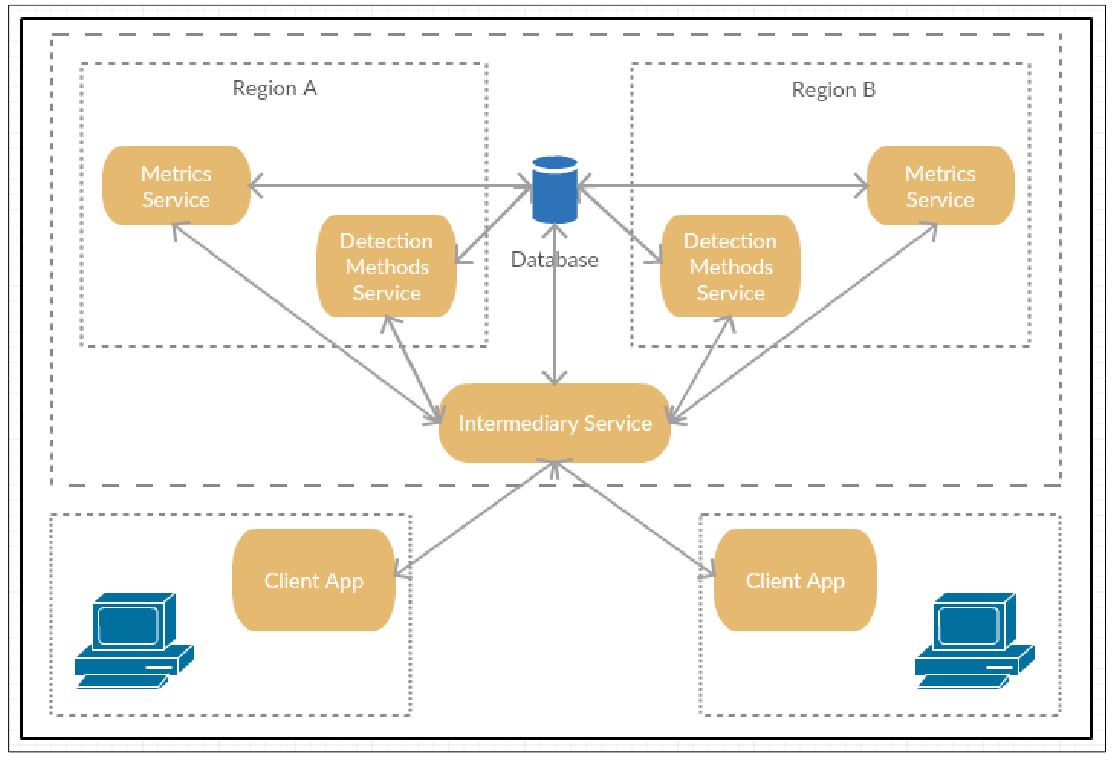
\includegraphics[width =\textwidth]{Chapter-2/Figures/schema.png}
\SourceOrNote{\textcite{beluzzo2018abordagem}}
\end{figure}
\FloatBarrier

The architecture diagram in Figure 4 begins in the Client App. It continues to the Intermediary Service, which will choose the processing service depending on the user's action and may choose "Request source code evaluation" and "Request application of design patterns."
The Intermediary Service process, when it receives a refactoring candidate from the ClientApp, sends the request to the Intermediary service, which sends the request to the Detection Methods Service, which scans the database for source code and obtains the refactoring candidates. Then, the candidates are returned to the intermediary service, which sends them to the Metrics Service for evaluation. 

After calculating the metrics, they are sent to the Intermediary service, which sends them back to the Client App to make the metrics and refactoring candidates available. If the user selects any candidate for refactoring, the Client App sends the requests to the Intermediary Service with the candidates to be refactored in the Detection Methods Service. Creates a project with the refactorings performed.

\textcite{beluzzo2018abordagem} was concerned with abstracting the tool so that an expansion could be performed without significant problems, but he defined no extension process.

\subsubsection{Internal structure}
\label{subsub-internal}

The architecture of a system is vital to work correctly, but all the heavy processing happens inside the services. A good design service will run with low memory and CPU, allowing it to work even on a small computer instance. The selection of refactoring candidates using RMT is described in \Cref{fig-candidates}.

\begin{figure}[ht!]
\SetCaptionWidth{\textwidth}
\caption{Sequence Diagram to Find Refactoring Candidates}
\label{fig-candidates}
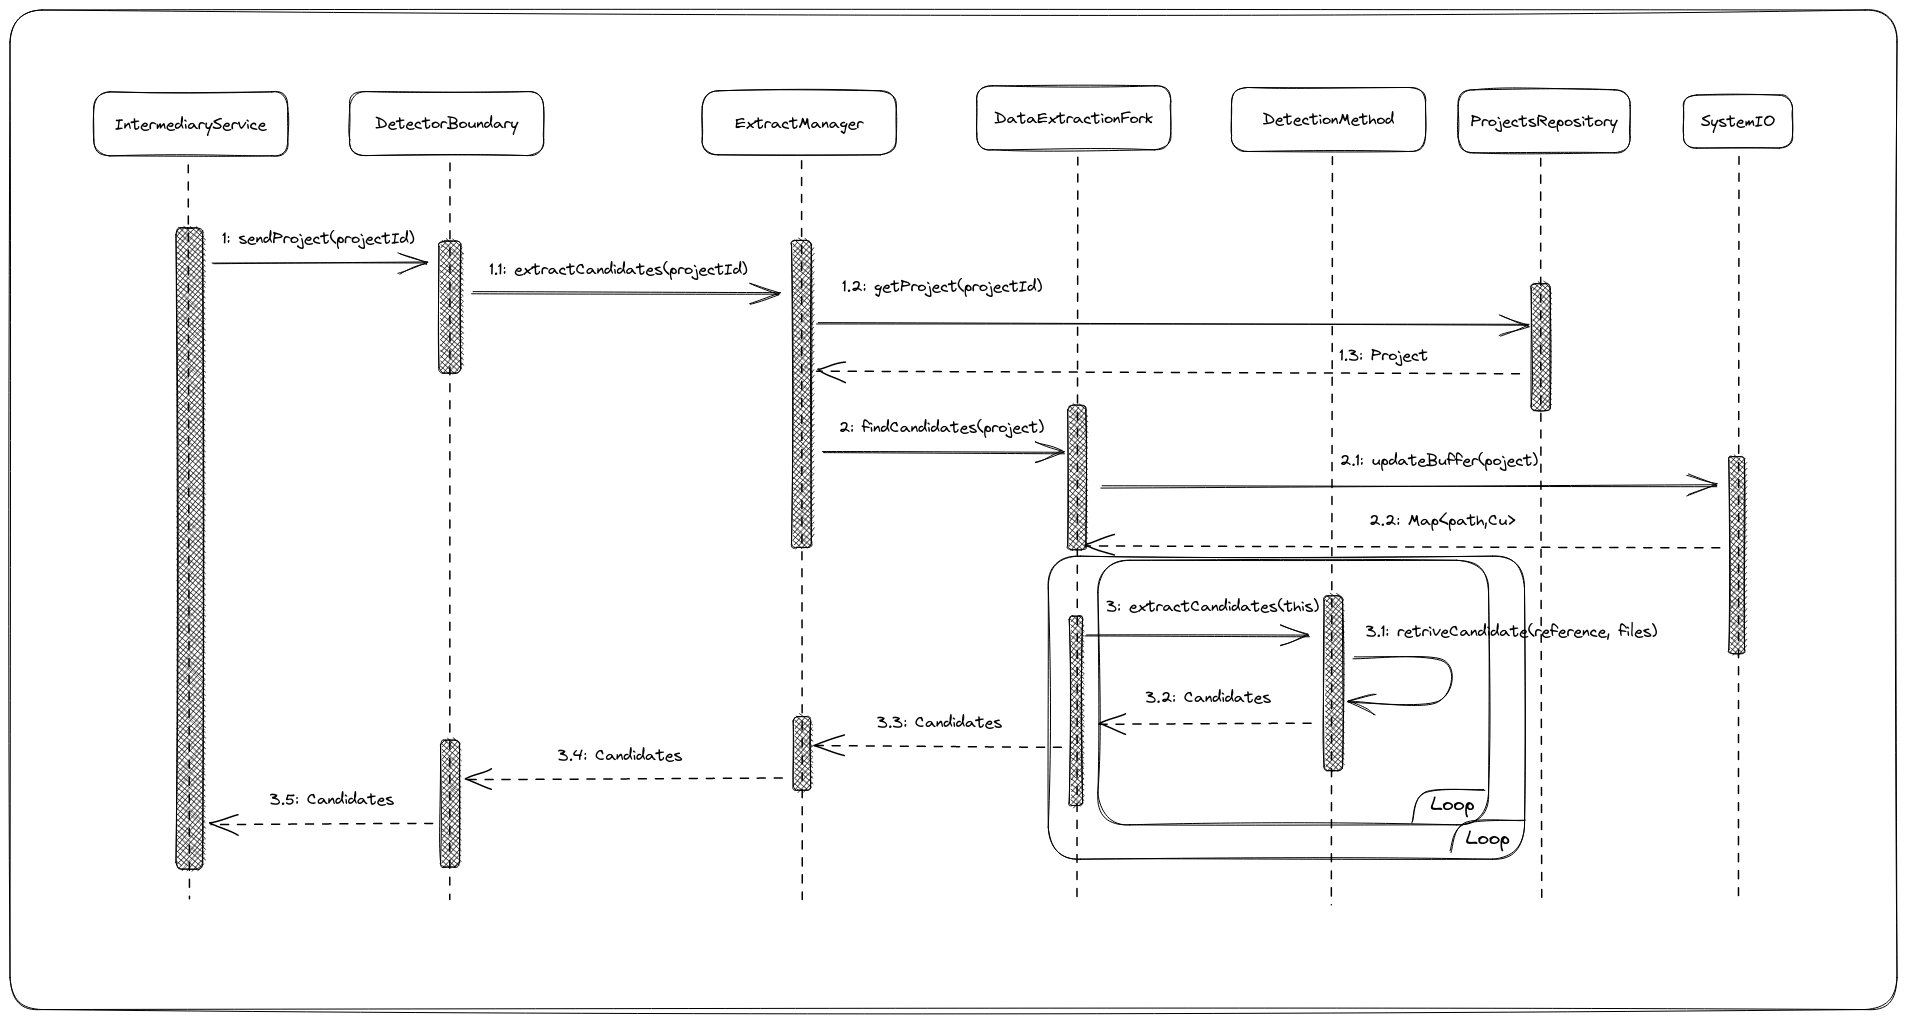
\includegraphics[width=160mm]{Chapter-2/Figures/candidates.png}
\SourceOrNote{Own authorship (2023)}
\end{figure}
\FloatBarrier

As described in the architecture, the intermediary service communicates with the other services, which is why the diagram starts there. After saving the project path and ID to the database, the intermediary service sends the ID to the DetectionService as step 1.

In the detection service, the class to receive information is the DetectionBoundary, which gets the ID and passes it ahead as a simple controller in Step 1.1. Step 2 sends the retrieved project to the DataExtractionFork.

The id is received by ExtractManager, an interface responsible for retrieving the project from the project repository and sending it to be parsed on the DataExtractionFork as Step 1.2.

The ProjectRepostiory is an interface with access to the database, which is consulted to retrieve the project information as a "Project" entity, completing Step 1.3.

The DataExtractionFork has direct access to the system io, which is used to retrieve the project from the file system; the project is saved as a zip file inflated to be parsed as a CompilationUnit and loaded into the memory to be sent to every implementation of the DetectionMethod as Step 2.1.

The DetectionMethod is an interface that abstracts the functionality of a new refactoring method; it receives an instance of the DataExtactionFork with the loaded files iterate over for every file and tries to detect if any pattern present on that method fits on the file and sends back the information via the stack finishing Step 3.1.

After selecting candidates, if the user decides to refactor, the system sends the chosen files to the intermediary service, and the process described in \Cref{fig-refactoring} starts.

\begin{figure}[ht!]
\SetCaptionWidth{\textwidth}
\caption{Sequence Diagram for Refactoring Candidates}
\label{fig-refactoring}
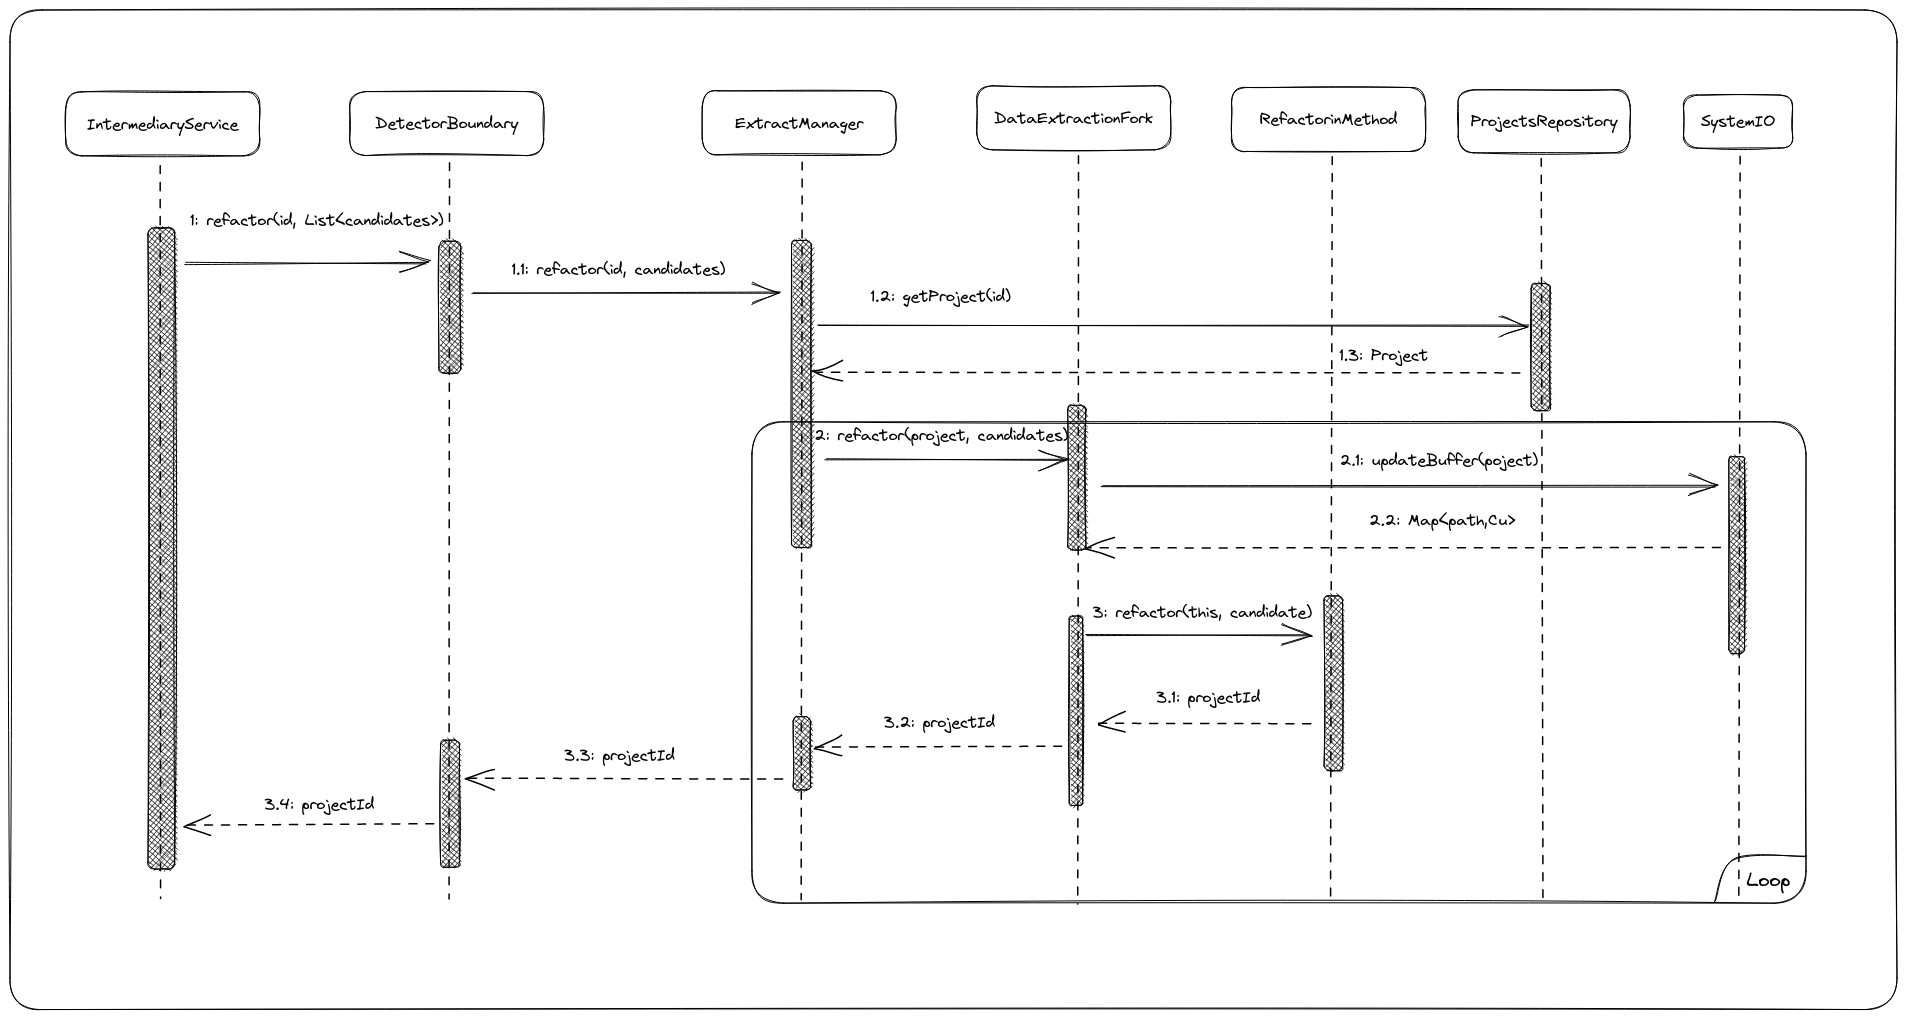
\includegraphics[width=160mm]{Chapter-2/Figures/refactoring.png}
\SourceOrNote{Own authorship (2023)}
\end{figure}
\FloatBarrier

As DetectionBoundry is the controller, it also revises the request to refactor with the user-selected classes and project ID to send to the ExtractManager as step 1.1.

The ExtractManager has the same functionality as on \Cref{fig-candidates}, retrieving the project from the database by the ProjectRepository (step 1.2) and sending it to the DataExtractionFork plus iterating it as step 2.

The DataExtractionFrok in Step 2.1 also has the same functionality. Still, every candidate in the project is called to return the same response every time since it inflates the zip file and converts it to the CompilationUnit entity. For Step 3, every candidate is sent to be refactored by the method defined on the candidate's face; after the process ends, the project ID is sent back via the stack.

\subsubsection{RMT Usage}
\label{sub-usage}

The main focus of explaining the usage of RMT is on the Client App, which is divided into three stages. The first step is to import the project, as shown in \Cref{fig-import}.

\begin{figure}[ht!]
\SetCaptionWidth{\textwidth}
\caption{Importing project on clientApp}
\label{fig-import}
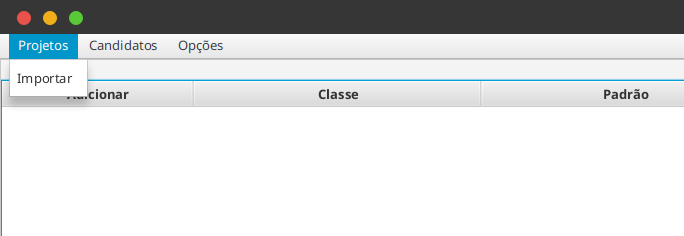
\includegraphics[width =100mm]{Chapter-2/Figures/import.png}
\SourceOrNote{Own authorship (2023)}
\end{figure}
\FloatBarrier


The second step is the project evaluation, giving feedback to the user, which can analyze additional information about the candidates for refactoring, such as class name, design pattern, and metrics, as shown in \Cref{fig-choose}.

\begin{figure}[ht!]
\SetCaptionWidth{\textwidth}
\caption{Selecting refactoring candidates}
\label{fig-choose}
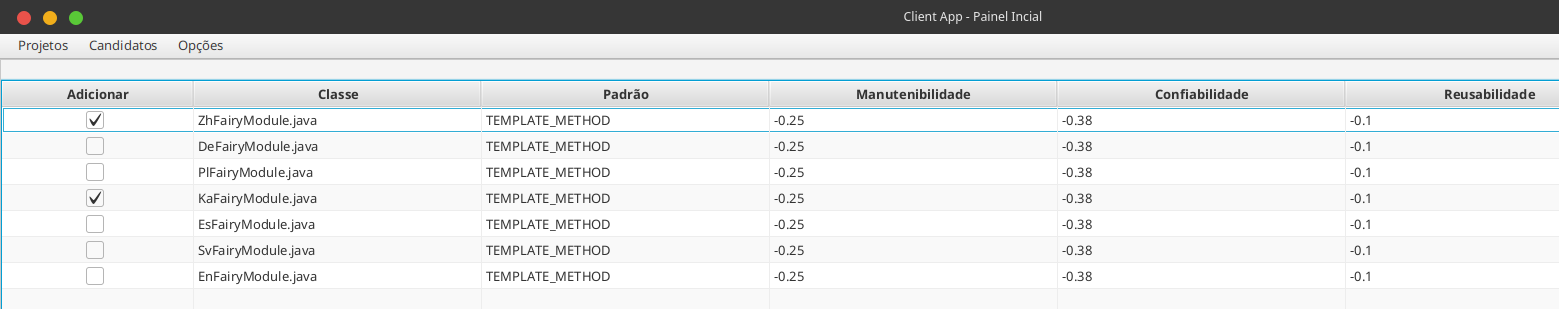
\includegraphics[width =\textwidth]{Chapter-2/Figures/choose.png}
\SourceOrNote{Own authorship (2023)}
\end{figure}
\FloatBarrier

In the third and last step, the user can choose the candidates to apply the refactoring after using it to a new project created and saved in a user-selected directory, as shown in \Cref{fig-refactor}.

\begin{figure}[ht!]
\SetCaptionWidth{\textwidth}
\caption{Applying refactoring to candidates}
\label{fig-refactor}
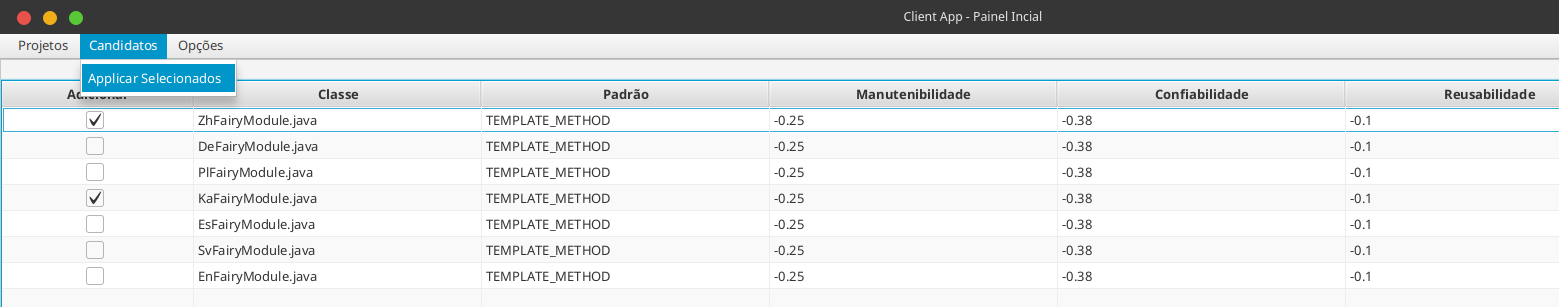
\includegraphics[width =\textwidth]{Chapter-2/Figures/refactor.png}
\SourceOrNote{Own authorship (2023)}
\end{figure}
\FloatBarrier

\subsubsection{RMT Limitations}
\label{subsub-limitation}
When testing, the RMT can spot some limitations, such as the time to execute and a blocking request that may cause slowness when many users try to use the tool; also related to the slowness is that for every project, analyses and refactoring the system open a zip file and parses every file to memory to check if it is a candidate, and repeating the same process when it's refactoring the files, besides the fact that accessing the disk takes time. For the interface, there is no explicit method of choosing between the same pattern applied by two approaches in the same class.

The prolonged execution time is caused by the strategy of finding where the refactoring can be applied and the refactor action because it is performed synchronously on the same thread. Each file is analyzed in order, causing slowness in significant projects with many files.

The lack of performance occurs when accessing the hard drive to retrieve the file for refactoring; for each refactoring step, the program parses the file and makes some changes to save it on disk; this could be solved by keeping the file in memory and changing it in memory.
The other problem implying the file system is that the architecture designed by \textcite{beluzzo2018abordagem} can be divided into regions, making it impossible to access the files with them being saved on one machine and the services being in another.

The blocking request is addressed when many users use the tool simultaneously, resulting in no more space for new connections. New users will increase latency, and users may receive an error and have to wait until someone refactors stops and opens space for a new connection. This problem mainly occurs because of the synchronous architecture on RMT based on an API composer (intermediary service) used to communicate with the other services via REST, providing dependency on the services as no intercommunication is made, acting as a load balancer, service registry, and discovery. The downside of REST communication is that latency increases with the number of concurrent clients \cite{Cebeci2020DesignOA}. 

When RMT shows the patterns of refactoring candidates, it may show two refactorings for the same design pattern and class, having only the metrics to choose from which will be applied; it lacks other ways to explain the difference between the method to the user to make a better decision.

The tool also lacks unit tests, which could guarantee that the logic created in the class is correct and could help with the refactoring, as it should not change the functionality, and the tests would have to continue working.

\section{Microservices Architecture}
\label{sec-microservices}
The microservices are used to create large and complex applications, as the model shown in \Cref{fig-architecture}, each application must be simple and independent; when the services are connected and working together, they become a system. As discussed in \textcite{microservices-comuni}, the application is fault-tolerant and more controllable than a monolithic architecture.

There are many architectures, such as synchronous RMT and asynchronous ones. The synchronous services wait for the response before ending the process; they usually use a direct connection over REST, RCP protocol, etc. \cite{microservices-comuni}. To implement a retry on sync services, the client service has to implement a strategy to handle the failure.

Asynchronous services do not wait for a response; the communication is non-block, so the service does not wait for the answer to end the process; it can be made with queues to handle communication. Those tools are RabbitMQ and Apache Kafka, among others \textcite{KARABEYAKSAKALLI2021111014}. Using queues can bring new features related to resilience; if a service is down, messages will be stored inside the queue and consumed when the service returns\cite{Cebeci2020DesignOA}. 

To work with retry, the queue has some implementations, such as visibility timeout, which is the time window in the message that is not visible to consumers; when the timeout is done and the message is not acknowledged, it becomes visible again, bringing resilience to the system; the downside is that it can duplicate the message over failure conditions \cite{ChenScalable}.

\section{Closing Remarks}
\label{sec2-remarks}
This chapter reported on the importance of refactoring, described the methods based on design patterns and refactoring tools, and explained some aspects of service architecture.

Refactoring is essential to keep the source code free from smells and to a quality standard. The main focus of refactoring is maintainability and reusability by maintaining the code as first designed and avoiding inserting new smells.

The importance of using a software refactoring tool was addressed to get the most out of refactoring without harming the work already done, highlighting that the RMT tool is the focus of this research.
The RMT tool integrates several methods for detecting and inserting design patterns in a single environment so that the application developer can apply them to their source code without having to use several refactoring tools that have refactoring tools for this purpose.

There are many types of software architecture, but we discuss the abilities of the async and sync applications, bringing both upsides and downsides. As \textcite{beluzzo2018abordagem} conducted a systematic review to find articles on refactoring with design patterns and tools, another research method, such as snowballing, could be used to ensure that there is no other tool like RMT.